\documentclass[11pt,a4paper]{article}
\usepackage[utf8]{inputenc}
\usepackage[margin=1in]{geometry}
\usepackage{xcolor}
\usepackage{listings}
\usepackage{tikz}
\usetikzlibrary{shapes.geometric, positioning, arrows.meta}
\usepackage[most]{tcolorbox}
\usepackage{enumitem}
\usepackage{hyperref}

% 🎨 Define Custom Color Palette
\definecolor{primaryblue}{HTML}{1A365D}   % Dark Navy for titles
\definecolor{accentblue}{HTML}{2B6CB0}    % Accent blue for subtitles
\definecolor{codegreen}{HTML}{2F855A}     % Green for comments/strings
\definecolor{codeorange}{HTML}{DD6B20}    % Orange for strings
\definecolor{codeblue}{HTML}{3182CE}      % Blue for keywords
\definecolor{codeyellow}{HTML}{D69E2E}    % Yellow for parameters/attributes
\definecolor{codegray}{HTML}{718096}      % Gray for metadata
\definecolor{bglight}{HTML}{F7FAFC}       % Soft light gray background
\definecolor{headerred}{HTML}{C53030}     % Red for JWT Header
\definecolor{payloadblue}{HTML}{2B6CB0}    % Blue for JWT Payload
\definecolor{signgreen}{HTML}{22543D}     % Green for JWT Signature

% 🛠️ Configure Listings for Colorful Code
\lstdefinelanguage{JavaScript}{
  keywords={const, let, var, function, return, import, from, export, default, async, await, try, catch, if, else, new},
  keywordstyle=\color{codeblue}\bfseries,
  ndkeywords={class, export, boolean, throw, implements, import, this, true, false, null},
  ndkeywordstyle=\color{codeyellow}\bfseries,
  identifierstyle=\color{black},
  sensitive=true,
  comment=[l]{//},
  morecomment=[s]{/*}{*/},
  commentstyle=\color{codegray}\itshape,
  stringstyle=\color{codeorange},
  morestring=[b]',
  morestring=[b]"
}

\lstset{
  language=JavaScript,
  backgroundcolor=\color{bglight},
  basicstyle=\small\ttfamily,
  breaklines=true,
  captionpos=b,
  frame=single,
  framesep=8pt,
  xleftmargin=10pt,
  framexleftmargin=10pt,
  rulecolor=\color{accentblue},
  showstringspaces=false,
  keepspaces=true,
  numbers=left,
  numberstyle=\tiny\color{codegray},
  numbersep=5pt,
  tabsize=2
}

% 📄 Page Setup
\hypersetup{
    colorlinks=true,
    linkcolor=accentblue,
    urlcolor=accentblue
}
\setlength{\parindent}{0pt}
\setlength{\parskip}{8pt}

\begin{document}

% 👑 Document Title Banner
\begin{tcolorbox}[
    colback=primaryblue,
    colframe=primaryblue,
    arc=6pt,
    left=15pt,
    right=15pt,
    top=20pt,
    bottom=20pt,
    coltext=white
]
    \centering
    {\huge\bfseries Understanding Authentication Tokens \& OAuth 2.0 \par}
    \vspace{8pt}
    {\large\itshape A Plain English, Real-World Guide to Digital Keys \& Web Security \par}
\end{tcolorbox}

\vspace{15pt}

% 📖 Section 1: What is a Token?
\section{🔑 What is an Authentication Token?}
In web development, an \textbf{Authentication Token} is a compact, digital piece of data that acts as a secure, temporary keycard. It proves to a server that a user has successfully logged in and is authorized to access specific files or perform certain actions.

Instead of transmitting the user's secret username and password with every single request (which would be highly insecure), the server checks this lightweight token to verify identity.

\subsection{🚗 Real-Life Analogy 1: The Theme Park Wristband}
Imagine you visit an amusement park like \textit{Prater} in Vienna:
\begin{enumerate}
    \item \textbf{Verification}: You stand in a long line at the entrance gate, show your identity card, and pay for a ticket.
    \item \textbf{Token Issuance}: Once confirmed, the gatekeeper attaches a \textbf{waterproof, tamper-evident wristband} to your arm.
    \item \textbf{Seamless Access}: For the rest of the day, you go to the roller coasters, water slides, and shows. You do not show your passport or credit card to every ride operator. You simply hold up your wristband. The operator looks at the wristband, checks that it is intact, and lets you on.
\end{enumerate}
In this scenario, the \textbf{wristband is the token}. It is temporary, signed (marked with the park's custom stamp), and limited in scope to that specific park.

\subsection{🏨 Real-Life Analogy 2: The Hotel Keycard}
When you check into a hotel:
\begin{enumerate}
    \item You present your ID card and credit card at the front desk.
    \item The receptionist encodes a plastic \textbf{magnetic keycard} (the token) and hands it to you.
    \item The card does not contain your name, password, or bank details. It contains a cryptographically encrypted code that is programmed to open only your room door (Scope) and only until 11:00 AM on your checkout day (Expiration).
\end{enumerate}

---

% 📖 Section 2: JSON Web Tokens (JWT)
\section{📦 Anatomy of a JSON Web Token (JWT)}
A common token format used in modern web applications (and in our \textbf{Vindobona Pro} codebase) is the \textbf{JSON Web Token (JWT)}. A JWT is composed of three parts separated by periods (\texttt{.}):

\begin{center}
    \textbf{\textcolor{headerred}{Header}} \textbf{.} \textbf{\textcolor{payloadblue}{Payload}} \textbf{.} \textbf{\textcolor{signgreen}{Signature}}
\end{center}

\begin{tcolorbox}[colback=bglight, colframe=accentblue, title=JWT Structure Breakdown]
\begin{itemize}[leftmargin=*]
    \item \textbf{\textcolor{headerred}{1. Header (Red)}}: Specifies the metadata of the token, indicating the algorithm used (e.g., HMAC SHA256) and the token type (JWT).
    \item \textbf{\textcolor{payloadblue}{2. Payload (Blue)}}: Contains the claims or core user data. In our app, this includes the user's database ID, username, and system permission role (e.g., \texttt{userId}, \texttt{username}, \texttt{role}). It also sets the expiration date (\texttt{exp}).
    \item \textbf{\textcolor{signgreen}{3. Signature (Green)}}: A secure cryptographic stamp created by taking the Header, the Payload, and running them through an encryption function using a private \textbf{secret key} (the \texttt{JWT\_SECRET}) stored safely on our server. If anyone alters the username or role in the Payload, the signature becomes invalid immediately, causing the server to reject the key.
\end{itemize}
\end{tcolorbox}

---

% 📖 Section 3: Code Implementation
\section{💻 OAuth \& Token Code Implementation}

Here is how our codebase interacts with these tokens.

\subsection{Generating and Signing the Token (Backend)}
In the Express auth router, once Google verifies the user's identity, we sign a custom JWT with an expiration of 2 hours, and redirect the user back to the React app:
\begin{lstlisting}
// File: backend/server/routes/auth.js
const token = jwt.sign(
    { 
        userId: req.user.id, 
        username: req.user.username, 
        role: req.user.role 
    },
    process.env.JWT_SECRET,
    { expiresIn: '2h' } // Token automatically expires in 2 hours
);

// Redirect the user back to React with the token as query parameters
const frontendUrl = process.env.FRONTEND_URL || "http://localhost:5173";
res.redirect(`${frontendUrl}?token=${token}&username=${req.user.username}`);
\end{lstlisting}

\subsection{Reading and Saving the Token (Frontend)}
When the React frontend boots up, a listener scans the address bar for the token, saves it into the browser's persistent memory (\texttt{localStorage}), and updates React state to trigger a login:
\begin{lstlisting}
// File: src/App.tsx
useEffect(() => {
  const params = new URLSearchParams(window.location.search);
  const urlToken = params.get('token');
  const urlUsername = params.get('username');

  if (urlToken && urlUsername) {
    // 💾 Save key inside browser memory
    localStorage.setItem('token', urlToken);
    localStorage.setItem('username', urlUsername);
    
    // ⚡ Update state to unlock the Dashboard shell
    setToken(urlToken);
    setUsername(urlUsername);

    // 🧹 Clean the address bar for security
    window.history.replaceState({}, document.title, window.location.pathname);
  }
}, []);
\end{lstlisting}

---

% 📖 Section 4: Architectural Flow Diagram
\section{📊 Architectural Token Exchange Diagram}
Below is a conceptual visualization of the token lifecycle during user login and API requests:

\vspace{15pt}
\begin{center}
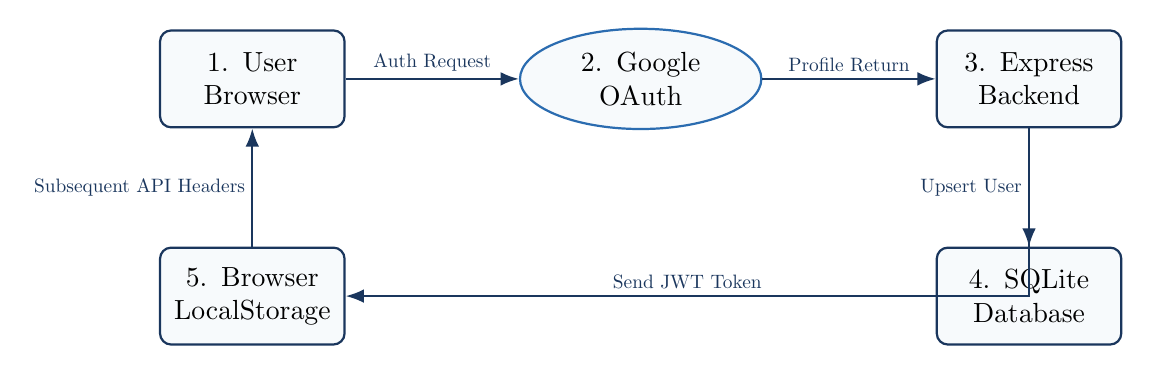
\begin{tikzpicture}[node distance=2.2cm, auto]
    % Styles
    \tikzstyle{block} = [rectangle, draw, fill=bglight, text width=6em, text centered, rounded corners, minimum height=3.5em, thick, draw=primaryblue]
    \tikzstyle{cloud} = [ellipse, draw, fill=bglight, text width=5.5em, text centered, rounded corners, minimum height=3.5em, thick, draw=accentblue]
    \tikzstyle{line} = [draw, -{Latex[scale=1.0]}, thick, primaryblue]
    
    % Nodes
    \node [block] (user) {1. User Browser};
    \node [cloud, right=2.2cm of user] (google) {2. Google OAuth};
    \node [block, right=2.2cm of google] (backend) {3. Express Backend};
    \node [block, below=1.5cm of backend] (db) {4. SQLite Database};
    \node [block, below=1.5cm of user] (storage) {5. Browser LocalStorage};

    % Paths
    \path [line] (user) -- node [above, scale=0.7] {Auth Request} (google);
    \path [line] (google) -- node [above, scale=0.7] {Profile Return} (backend);
    \path [line] (backend) -- node [left, scale=0.7] {Upsert User} (db);
    \path [line] (backend) |- node [above, near end, scale=0.7] {Send JWT Token} (storage);
    \path [line] (storage) -- node [left, scale=0.7] {Subsequent API Headers} (user);
\end{tikzpicture}
\end{center}
\vspace{10pt}

\begin{tcolorbox}[colback=primaryblue!5, colframe=primaryblue, title=Key Security Takeaways]
\begin{itemize}[leftmargin=*]
    \item \textbf{Token Storage}: Storing the token in \texttt{localStorage} keeps users logged in even if they refresh the tab.
    \item \textbf{State Cleaning}: Clearing the address bar using \texttt{window.history.replaceState} prevents the token from leaking via browser histories or shoulder surfing.
    \item \textbf{Stateless Verification}: The backend doesn't need to look up passwords on every database query; it checks the mathematical signature of the JWT token to verify authenticity in milliseconds.
\end{itemize}
\end{tcolorbox}

\end{document}
